\documentclass[11pt]{article}
\usepackage{fullpage, graphicx}
\usepackage{url}
\usepackage{amsmath}


\begin{document}
\thispagestyle{empty}
\parindent 0pt
\vfill
\large

\pagebreak[4]
\begin{center}
\LARGE{\bf \textsf{Cover Sheet}} \\*[4ex]
\end{center}

\textbf{Assignment Submission } Fill in and include this cover sheet with each of your assignments. Assignments are due at 11:59pm. All students (SCPD and non-SCPD) must submit their homeworks via GradeScope (\url{http://www.gradescope.com}). Students can typeset or scan their homeworks. Make sure that you answer each question on a separate page. Students also need to upload their code at \url{http://snap.stanford.edu/submit}. Put all the code for a single question into a single file and upload it. Please do not put any code in your GradeScope submissions.
\\
\\
\textbf{Late Day Policy } Each student will have a total of {\em two} free late periods. {\em One late period expires at the start of each class.} (Homeworks are usually due on Thursdays, which means the first late periods expires on the following Tuesday.) Once these late periods are exhausted, any assignments turned in late will be penalized 50\% per late period. However, no assignment will be accepted more than {\em one} late period after its due date.
\\
\\
\textbf{Honor Code } We strongly encourage students to form study groups. Students may discuss and work on homework problems in groups. However, each student must write down their solutions independently i.e., each student must understand the solution well enough in order to reconstruct it by him/herself.  Students should clearly mention the names of all the other students who were part of their discussion group. Using code or solutions obtained from the web (github/google/previous year solutions etc.) is considered an honor code violation. We check all the submissions for plagiarism. We take the honor code very seriously and expect students to do the same.

\vfill
\vfill

{\Large
\textbf{Your name:} \hrulefill \\
\textbf{Email:} \underline{\hspace*{7cm}} \textbf{SUID:} \hrulefill\\*[2ex] }
Discussion Group (People with whom you discussed ideas used in your answers): \\
Discuss with Jing Wang with Question4(c)
\\\\
On-line or hardcopy documents used as part of your answers: \\
Use the idea in the below response for sorting hashtable in question 1\\
http://stackoverflow.com/questions/109383/sort-a-mapkey-value-by-values-java?rq=1\\
\\
\vfill


\vfill

I acknowledge and accept the Honor Code.\\*[3ex]
\bigskip
\textit{(Signed)}\hrulefill
% If you are not printing this document out, just type your initials above

\vfill
\vfill

\pagebreak[4]
\begin{center}
\LARGE{\bf \textsf{CS246: Mining Massive Datasets}}\\ {\bf \textsf{Homework 1}}
\\*[4ex]
\end{center}

\section*{Answer to Question 1}
Here is a brief description of the algorithm:\\
\\
\textbf{Map:}\\
At this step for each line of data, assume there is a simple line of data like this:
$$
    (N_{i}: N_{j}, N_{k}, N_{m})
$$
Take its values and construct pairs, those pairs represents they share the same friend $N_i$. Then we construct:
$$
 (N_j: (N_k, 1)), (N_j: (N_m, 1)), (N_k: (N_j, 1)), (N_k: (N_m, 1)), (N_m: (N_j, 1)), (N_m: (N_k, 1))
$$
Here $1$ means, the value can be recommended to the key. Since there may have possibility that they are already friends,
therefore based on this line we can construct:
$$
 (N_i:(N_j, 0)), (N_i:(N_k, 0)), (N_i:(N_m, 0))
$$
Here $0$ means the value cannot be recommended to the key.\\
\\
\textbf{Reduce:}\\
Each reducer has two tasks to do. For the value tuples,
if the value contains $1$ this value will be added to a hash table and count how many this value appears.
On the other hand if the value tuple contains $0$, this value will be added to a set.
This set keeps a record who is already a friend of the key.
After iterate all the value tuple, name in the set will be excluded from the hash table.\\
\\
The hash table will in the end be sorted and output its top 10 records.\\
\\
924	439,2409,6995,11860,15416,43748,45881\\
8941 8943,8944,8940\\
8942 8939,8940,8943,8944\\
9019	9022,317,9023\\
9020	9021,9016,9017,9022,317,9023\\
9021	9020,9016,9017,9022,317,9023\\
9022	9019,9020,9021,317,9016,9017,9023\\
9990	13134,13478,13877,34299,34485,34642,37941\\
9992	9987,9989,35667,9991\\
9993	9991,13134,13478,13877,34299,34485,34642,37941\\

\pagebreak[4]
\section*{Answer to Question 2(a)}
Ignoring $Pr(B)$ can lead to recommen items that are not very frequent;
or item $B$ has very high support then it shows up in nearly every basket.
If this item has very high support confidence $conf(A\rightarrow B)$ is not very useful.\\
\\
While lift and conviction consider support in their formula. When $Pr(B)$ gets higher,
there will be a high support $S(B)$. Then $lift(A\rightarrow B) = \frac{conf(A\rightarrow B)}{S(B)}$
will get a smaller value. Conviction is similar, a high support value $S(B)$ will make conviction smaller.
Therefore, both conviction and lift consider $Pr(B)$ and reflects how offer $A$ and $B$ are together due to the existence of $A$.

\pagebreak[4]
\section*{Answer to Question 2(b)}
\textbf{confidence: }\\
\begin{equation}
    conf(A\rightarrow B) = Pr(B|A)
\end{equation}
\begin{equation}
    conf(B\rightarrow A) = Pr(A|B)
\end{equation}
It is very easy to see they are not necessarily the same.
For example there are two baskets $\{A, B\}, \{A\}$ and assume $N=1$.
$conf(A\rightarrow B) = 0.5$ and $conf(B\rightarrow A) = 1$.
Confidence is not symmetrical.\\
\\
\textbf{lift: }
\begin{equation}
\begin{aligned}
    lift(A\rightarrow B) & = \frac{conf(A\rightarrow B)}{S(B)}\\
    & = \frac{Pr(B|A)}{Support(B)/N}\\
    & = \frac{Support(AB)/Support(A)}{Support(B)/N} = \frac{Support(AB)/Support(B)}{Support(A)/N}\\
    & = \frac{Pr(A|B)}{Support(A)/N}\\
    & = \frac{conf(B\rightarrow A)}{S(A)}\\
    & = lift(B\rightarrow A)
\end{aligned}
\end{equation}
Therefore lift is symmetrical.\\
\\
\textbf{conviction: }
\begin{equation}
\begin{aligned}
    conviction(A\rightarrow B) & = \frac{1 - support(B)/N}{1 - conf(A\rightarrow B)}\\
    & = \frac{1 - support(B)/N}{1 - Pr(B|A)}\\
    & = \frac{1 - support(B)/N}{1 - Support(AB)/Support(A)}
\end{aligned}
\end{equation}
\begin{equation}
\begin{aligned}
    conviction(B\rightarrow A) & = \frac{1 - support(A)/N}{1 - conf(B\rightarrow A)}\\
    & = \frac{1 - support(A)/N}{1 - Pr(A|B)}\\
    & = \frac{1 - support(A)/N}{1 - Support(AB)/Support(B)}
\end{aligned}
\end{equation}
It can be seen that above two equations do not necessarily equal to each other.
For example there are two baskets $\{A, B\}, \{A\}$ and assume $N=1$.
$conviction(A\rightarrow B) = 0$ and $conviction(B\rightarrow A) = -\infty$.
Therefore, conviction is not symmetrical.

\pagebreak[4]
\section*{Answer to Question 2(c)}
\textbf{confidence: }\\
\begin{equation}
    conf(A\rightarrow B) = Pr(B|A) = \frac{support(AB)}{support(A)}
\end{equation}
$support(AB) \leq support(A)$ and $conf(A\rightarrow B)$ gets its maxima only when $support(AB) = support(A)$.
This means this rules hold $100\%$ of the time. Therefore, confidence is desirable.\\
\\
\textbf{lift: }
\begin{equation}
\begin{aligned}
    lift(A\rightarrow B) & = \frac{conf(A\rightarrow B)}{S(B)}\\
    & = \frac{Pr(B|A)}{Support(B)/N}\\
    & = \frac{Support(AB)/Support(A)}{Support(B)/N}
\end{aligned}
\end{equation}
When the rules hold $100\%$ of the time, have $support(AB) = support(A)$.
However $support(B)$ varies, then lift cannot guarantee to reach its maxima.
Therefore, lift is not desirable.
\\
\textbf{conviction: }
\begin{equation}
\begin{aligned}
    conviction(A\rightarrow B) & = \frac{1 - support(B)/N}{1 - conf(A\rightarrow B)}\\
    & = \frac{1 - support(B)/N}{1 - Pr(B|A)}\\
    & = \frac{1 - support(B)/N}{1 - Support(AB)/Support(A)}
\end{aligned}
\end{equation}
$conviction(A\rightarrow B)$ increases with $support(A)$ increasing.
$conviction(A\rightarrow B)$ reaches its maxima $+\infty$ when $support(AB) = support(A)$. This imply rules hold $100\%$ of the time.
Therefore, conviction is desirable.

\pagebreak[4]
\section*{Answer to Question 2(d)}
\begin{equation*}
\begin{aligned}
& conf(DAI93865\rightarrow FRO40251) = 1.0\\
& conf(GRO85051\rightarrow FRO40251) = 0.999176276771005\\
& conf(GRO38636\rightarrow FRO40251) = 0.9906542056074766)\\
& conf(ELE12951\rightarrow FRO40251) = 0.9905660377358491)\\
& conf(DAI88079\rightarrow FRO40251) = 0.9867256637168141)
\end{aligned}
\end{equation*}

\pagebreak[4]
\section*{Answer to Question 2(e)}
\begin{equation*}
\begin{aligned}
& conf(DAI23334,ELE92920\rightarrow DAI62779) = 1.0\\
& conf(DAI31081,GRO85051\rightarrow FRO40251) = 1.0\\
& conf(DAI55911,GRO85051\rightarrow FRO40251) = 1.0\\
& conf(DAI62779,DAI88079\rightarrow FRO40251) = 1.0\\
& conf(DAI75645,GRO85051\rightarrow FRO40251) = 1.0
\end{aligned}
\end{equation*}


\pagebreak[4]
\section*{Answer to Question 3(a)}
The probability of getting don`t know is:\\
\begin{equation}
    P = \frac{n-m}{n}\frac{n-m-1}{n-1}...\frac{n-m-k+1}{n-k+1} =\frac{\frac{(n-m)!}{(n-m-k)!}}{\frac{n!}{(n-k)!}}
\end{equation}
It is easy to see:
\begin{equation}
    P = \frac{\frac{(n-m)!}{(n-m-k)!}}{\frac{n!}{(n-k)!}} \leq (\frac{n-m}{n})^k
\end{equation}
Then let`s prove:
\begin{equation}
    (\frac{n-m}{n})^k \leq (\frac{n-k}{n})^m
\end{equation}
It can be rewriten as:
\begin{equation}
    (n-m)^k(n)^{m-k} \leq (n-k)^m
\end{equation}
Use the AM–GM inequality and also given $m\geq k$:
\begin{equation}
    (n-m)^k(n)^{m-k} \leq (\frac{k(n-m)+(m-k)n}{m-k+k})^{m-k+k} = (n-k)^{m}
\end{equation}
Therefore, when $m=k$ this inequality gets its equal sign:
\begin{equation}
    P  \leq (\frac{n-m}{n})^k \leq (\frac{n-k}{n})^m
\end{equation}

\pagebreak[4]
\section*{Answer to Question 3(b)}
Use the result from 3(a) and assume:
\begin{equation*}
    P = (\frac{n-k}{n})^m = (1 - \frac{1}{n/k})^m = (1 - \frac{1}{n/k})^{n/k\frac{m}{n/k}}
\end{equation*}
Since $n$ is much larger than $k$, therefore we can approximate as following:
\begin{equation*}
    P = (\frac{n-k}{n})^m = (1 - \frac{1}{n/k})^{n/k\frac{m}{n/k}} \approx e^{-\frac{m}{n/k}}
\end{equation*}
Therefore,
\begin{equation*}
    -\frac{m}{n/k} = -10
\end{equation*}
\begin{equation}
    k = 10\frac{n}{m}
\end{equation}

\pagebreak[4]
\section*{Answer to Question 3(c)}
a) Below is an example of the matrix:
\begin{equation*}
\begin{bmatrix}
    1 & 1\\
    0 & 1\\
    1 & 0\\
    0 & 0
\end{bmatrix}
\end{equation*}
b) The Jaccard Similarity for the two columns is $1/3$.\\
\\
c) There are three cyclic permutation and the resulting signatures of them are:
$(0, 0)$, $(2, 1)$, $(2, 0)$ and $(0, 0)$. As can be seen only one of them has the same minhash value.
Therefore, the probability is $1/2$

\pagebreak[4]
\section*{Answer to Question 4(a)}
Since $g$ is a $k$ way And-construct based on $h$,
then we can say $G$ is $(\lambda,c\lambda, p_1^k, p_2^k)$-sensitive.
Apply markov`s inequality:
\begin{equation}
\begin{aligned}
Pr[\sum_{j=1}^L|T\cap W_j|\geq3L] & \leq \frac{E(\sum_{j=1}^L|T\cap W_j|)}{3L}\\
& = \frac{Lnp_2^k}{3L} = \frac{np_2^k}{3}\\
&  = \frac{np_2^{log_{1/p_2}^n}}{3} = \frac{np_2^{log_{p_2}^{1/n}}}{3} = \frac{1}{3}
\end{aligned}
\end{equation}

\pagebreak[4]
\section*{Answer to Question 4(b)}
\begin{equation}
\begin{aligned}
Pr[\forall1\leq j\leq L, g_j(x^{*})\neq g_j(z)] & = (1-p_i^k)^L\\
& = (1-p_1^{\log_{p_2}^{1/n}})^{n^{\frac{log{1/p_1}}{log{1/p_2}}}}\\
& = (1-p_1^{\log_{p_1}^{1/n}\log_{p_2}^{p_1}})^{n^{\log_{p_2}^{p_1}}}\\
& = (1-{\frac{1}{n^{\log_{p_2}^{p_1}}}})^{n^{\log_{p_2}^{p_1}}}
\end{aligned}
\end{equation}
Recall that when $x>1$ the following function increase with $x$ and has a limit $1/e$:
\begin{equation}
(1 - 1/x)^x < 1/e
\end{equation}
Since $n^{\log_{p_2}^{p_1} > 1}$, therefore,
\begin{equation}
Pr[\forall1\leq j\leq L, g_j(x^{*})\neq g_j(z)] < 1/e
\end{equation}

\pagebreak[4]
\section*{Answer to Question 4(c)}
This question can be translated as the probability that exists a point $x'$ such that it is the correct neighbor and it hashed to the same value as $z$.
There exists two condition in order to get correct neighbor, that is: (1)
there exists point which is the correct neighbor and at the same time hased to same value as $z$;
(2) for the point hased to the same value as $z$ it shoud have distance less than $c\lambda$.\\
\\
Therefore the probability for existing a point $x'$:
\begin{equation*}
\begin{aligned}
    Pr[\exists1\leq j\leq L, g_j(x^{*}) = g_j(z),d(x^{*}, z)\leq c\lambda]
    & \geq Pr[\forall1\leq j\leq L, g_j(x^{*}) = g_j(z)|d(x^{*}, z)\leq \lambda]\\
    & \times Pr[\forall x^{*}\in X | \forall j, g_j(x^{*}) = g_j(z), d(x^{*}, z) < c\lambda]\\
    & \geq (1 - Pr[\forall1\leq j\leq L, g_j(x^{*})\neq g_j(z)]|d(x^{*}, z)\leq \lambda)\\
    & \times (1 - Pr[\forall x^{*}\in X | \forall j, g_j(x^{*}) = g_j(z), d(x^{*}, z)\geq c\lambda])\\
    & \geq (1 - 1/e)(1 - 1/3)\\
    & = 2/3(1 - 1/e)
\end{aligned}
\end{equation*}
Use the result from 4(b), we find with probability greater than $2/3(1 - 1/e)$,
the reported point is an actual $(c, \lambda)$-ANN.

\pagebreak[4]
\section*{Answer to Question 4(d)}
Average search time for LSH is 0.219991 seconds.\\
Average search time for Linear is 1.921050 seconds.\\

The figure seems kind stochastic but we can still see when increasing $L$ the error decreases
because it will give a better guarantee on the candidates.
For $K$, the error seems to increase with the increase of key bits.
\begin{figure}[h]
\center
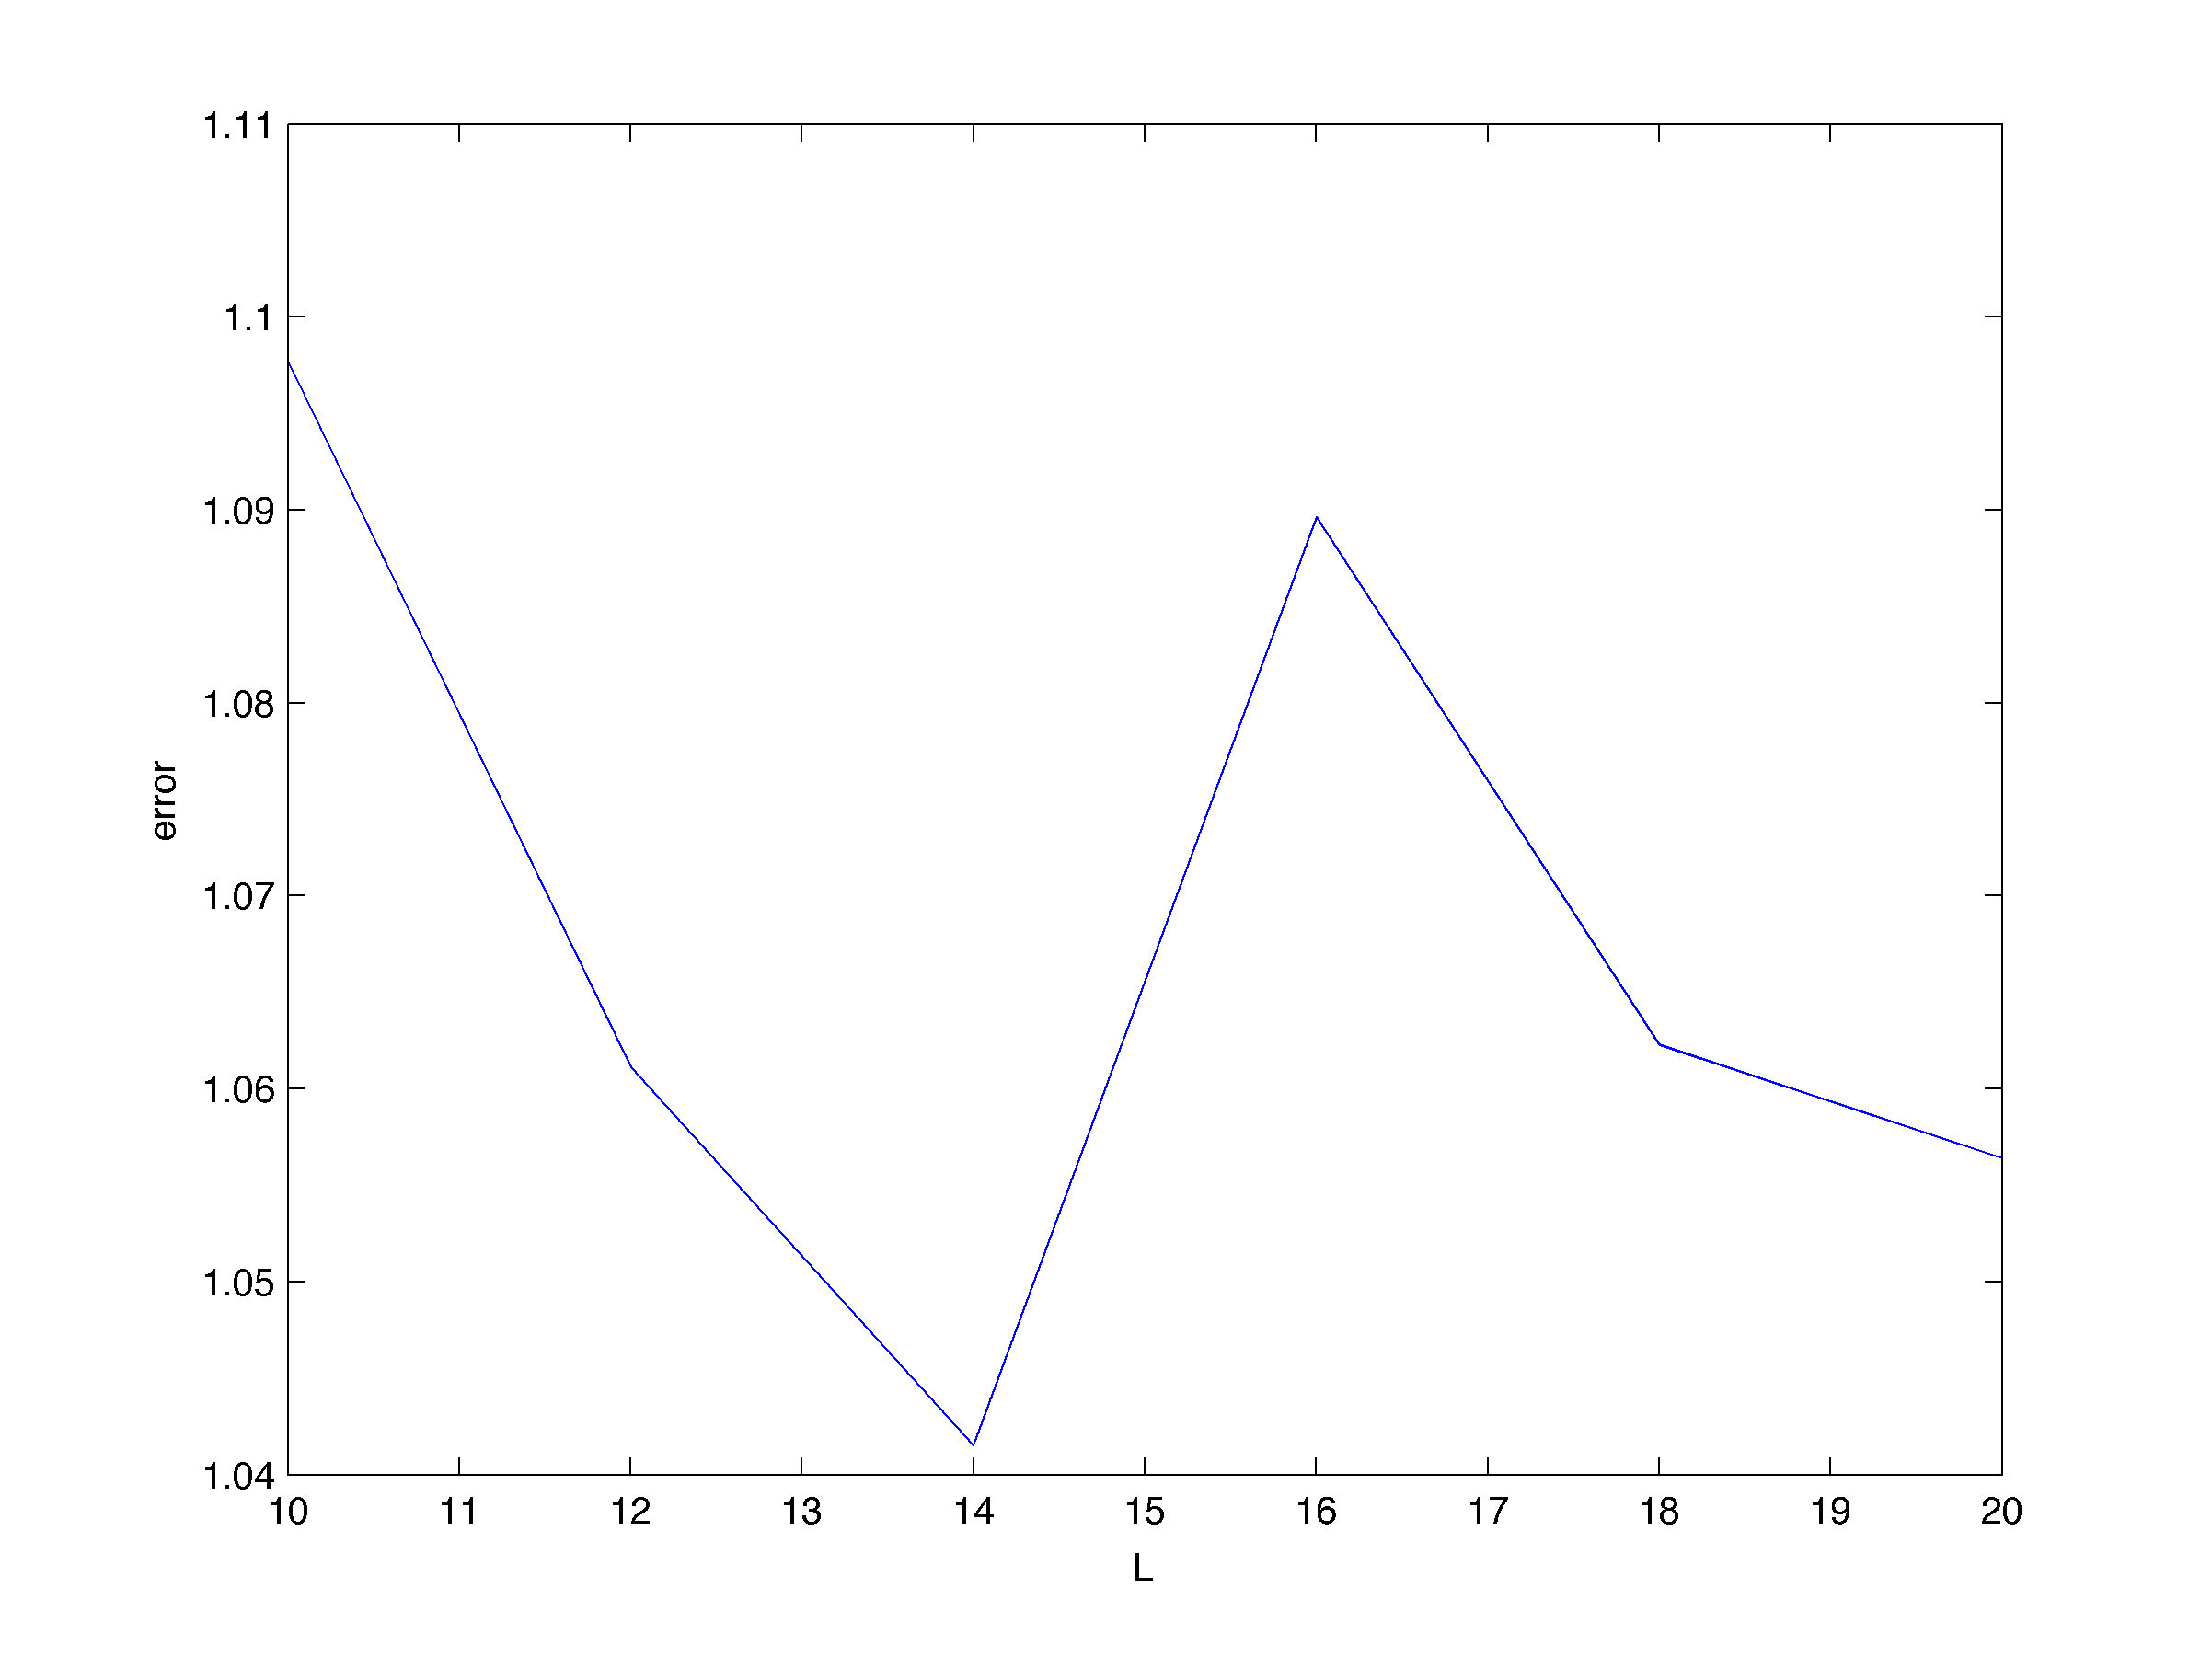
\includegraphics[scale=0.5]{L_error.png}
\end{figure}

\begin{figure}[h]
\center
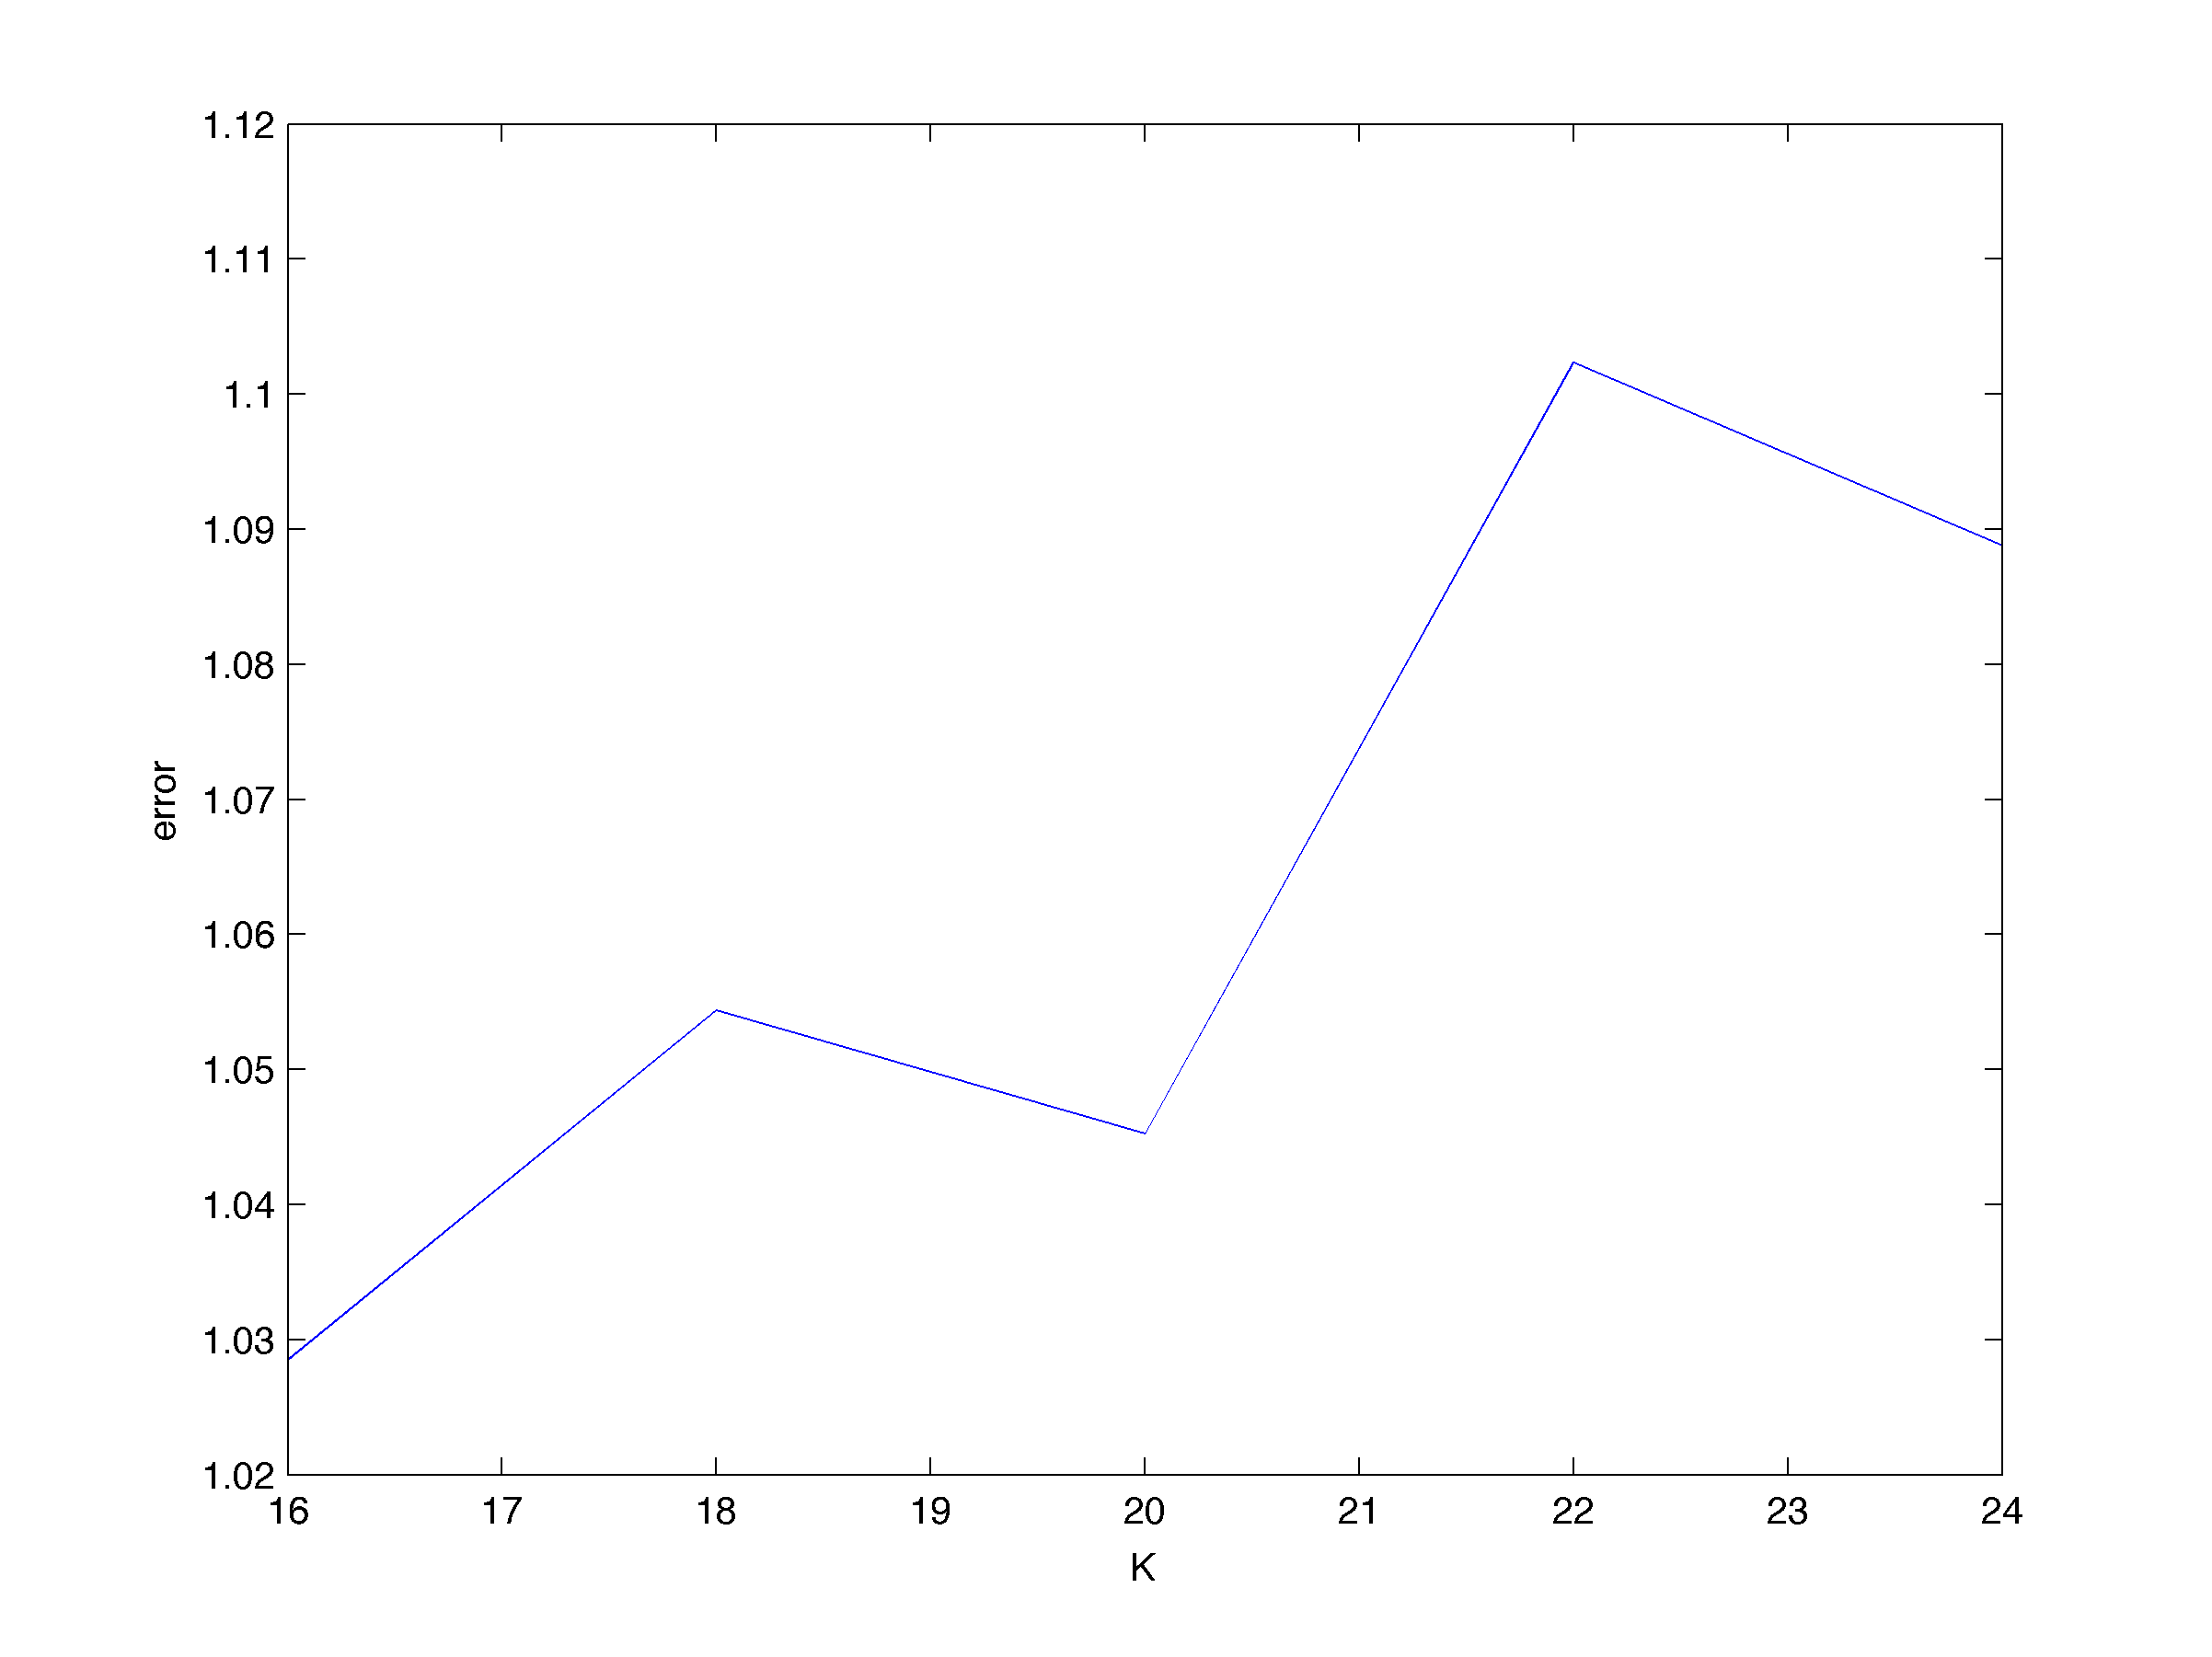
\includegraphics[scale=0.5]{K_error.png}
\end{figure}

\pagebreak[4]
\section*{Continued Answer to Question 4(d)}
We can see LSH search and linear search produce some common image patches.
Other image patches more or less have similar pattern.
Visually we can not say which methods do better
but both of the methods produce images that have some similarities to the original images.
\begin{figure}[h]
\center
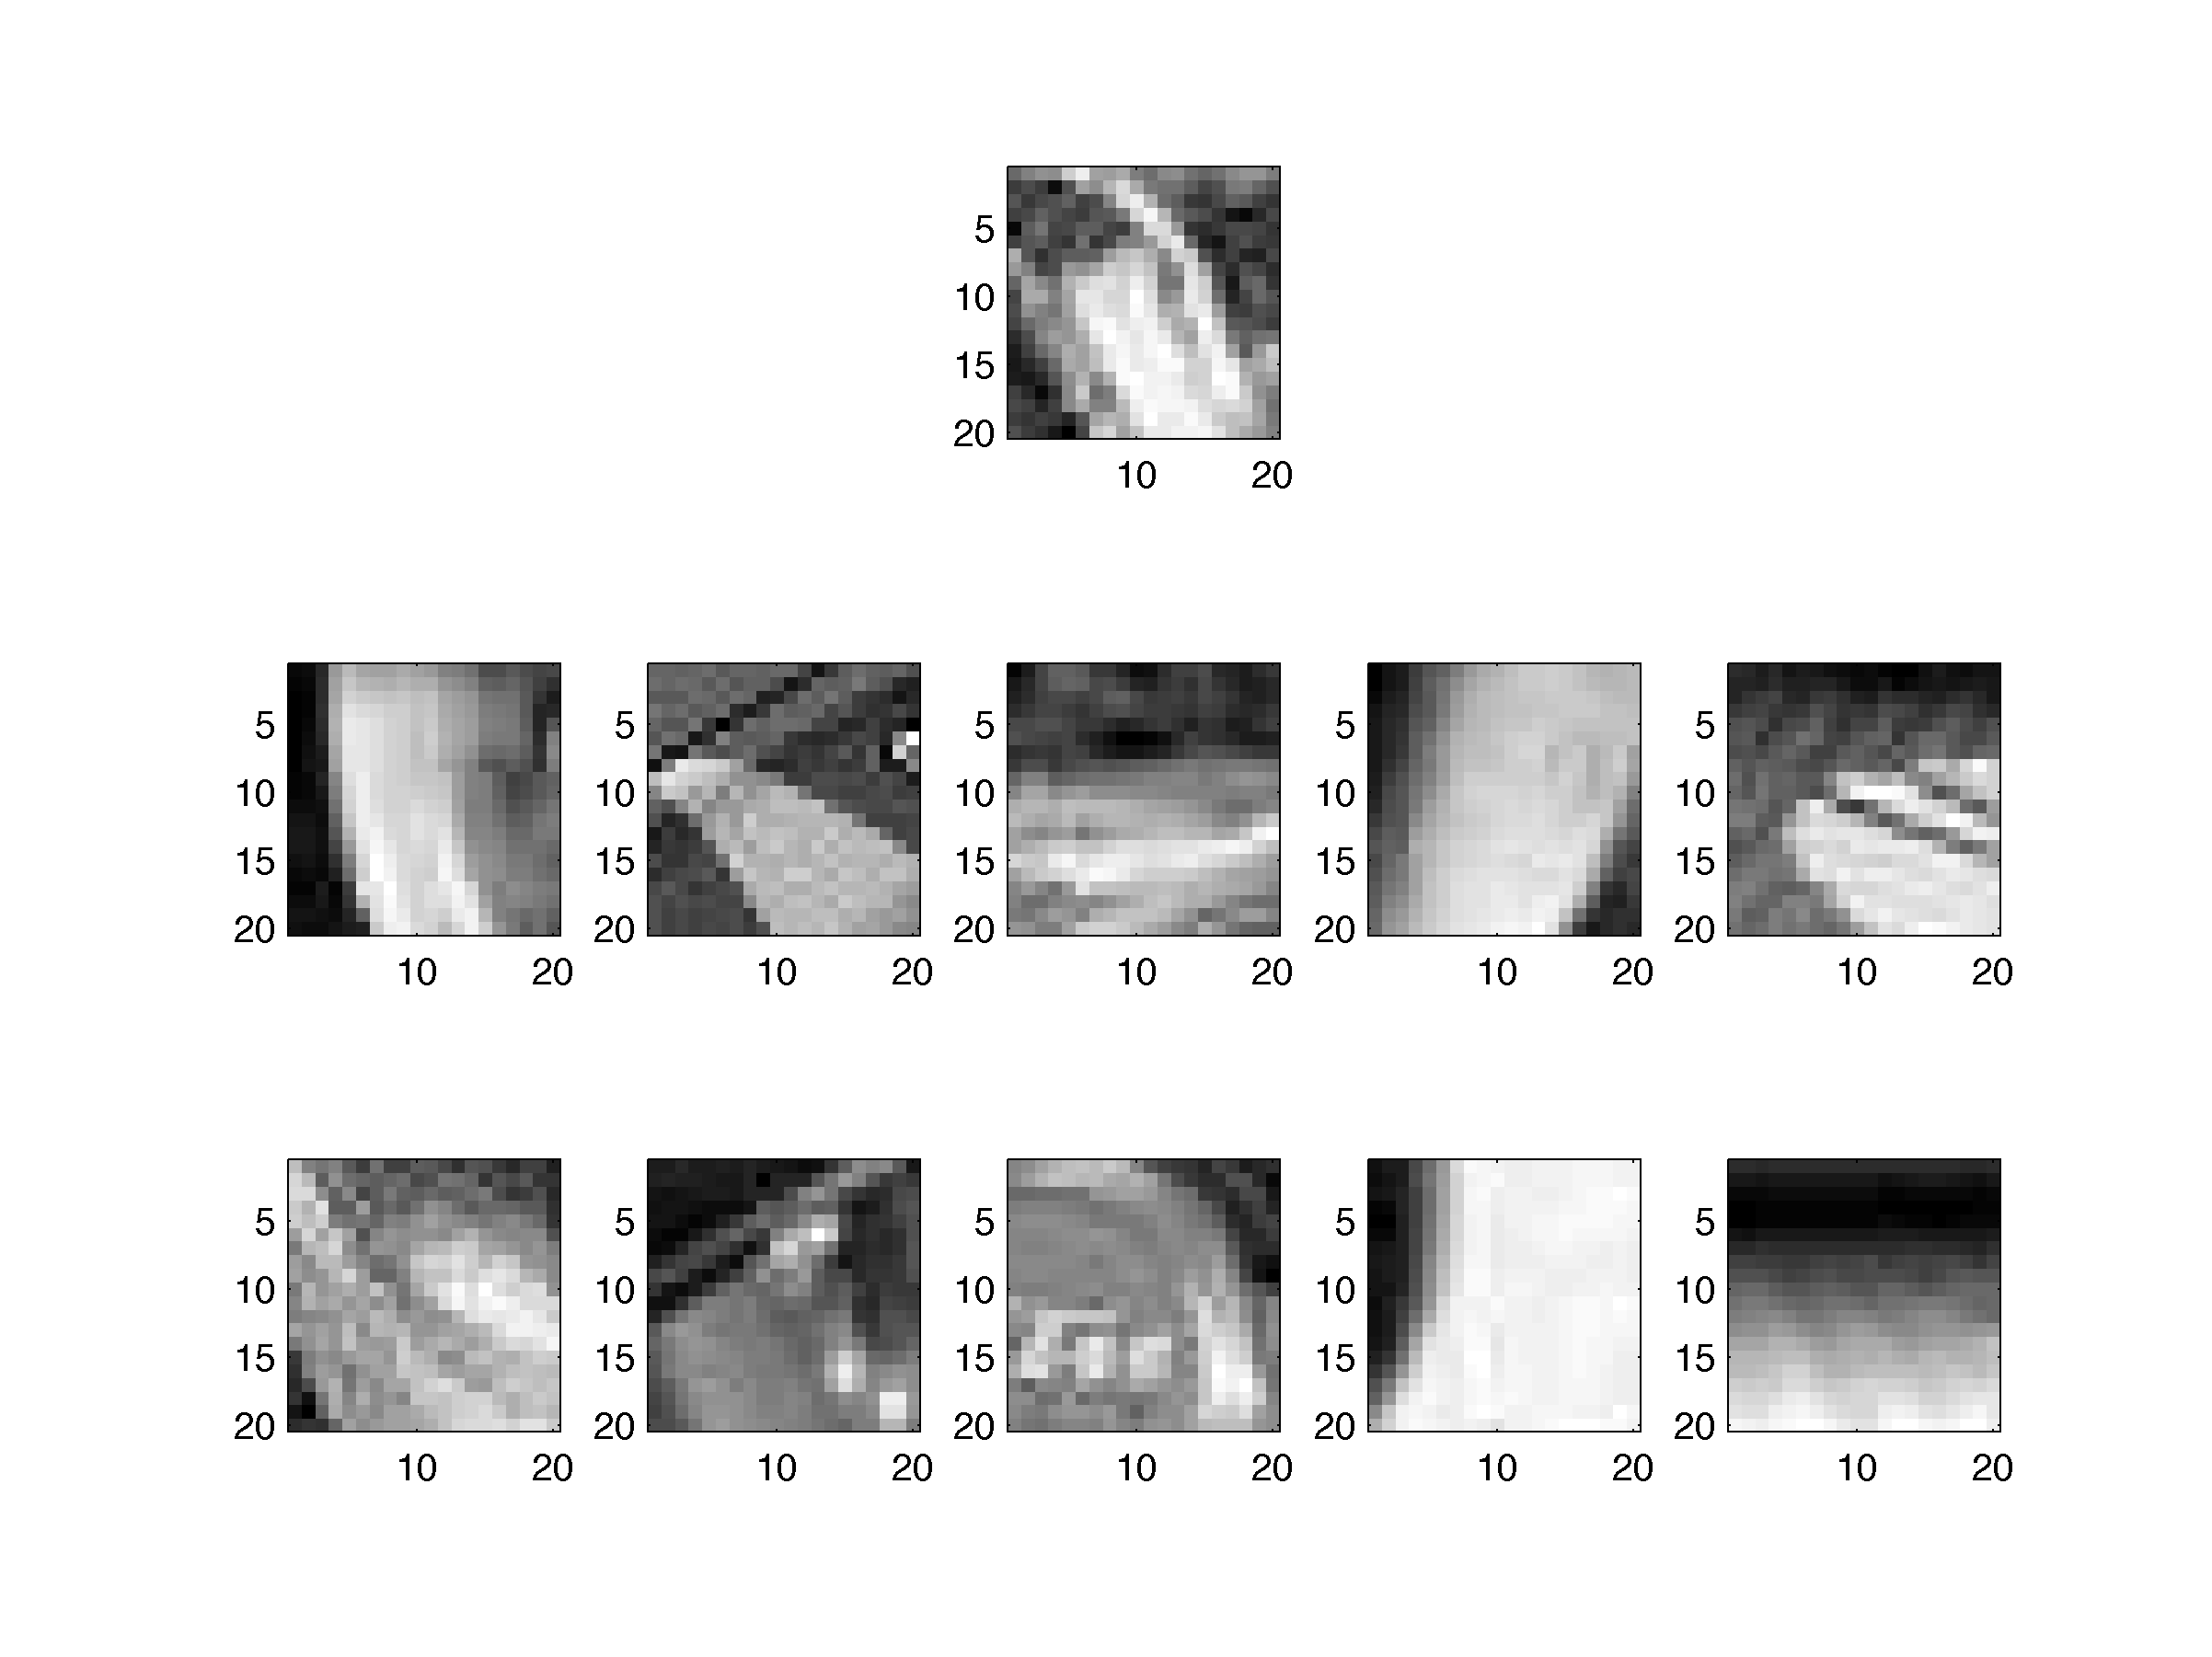
\includegraphics[scale=0.45]{LSH_negihbor.png}
\caption{LSH search}
\end{figure}

\begin{figure}[h]
\center
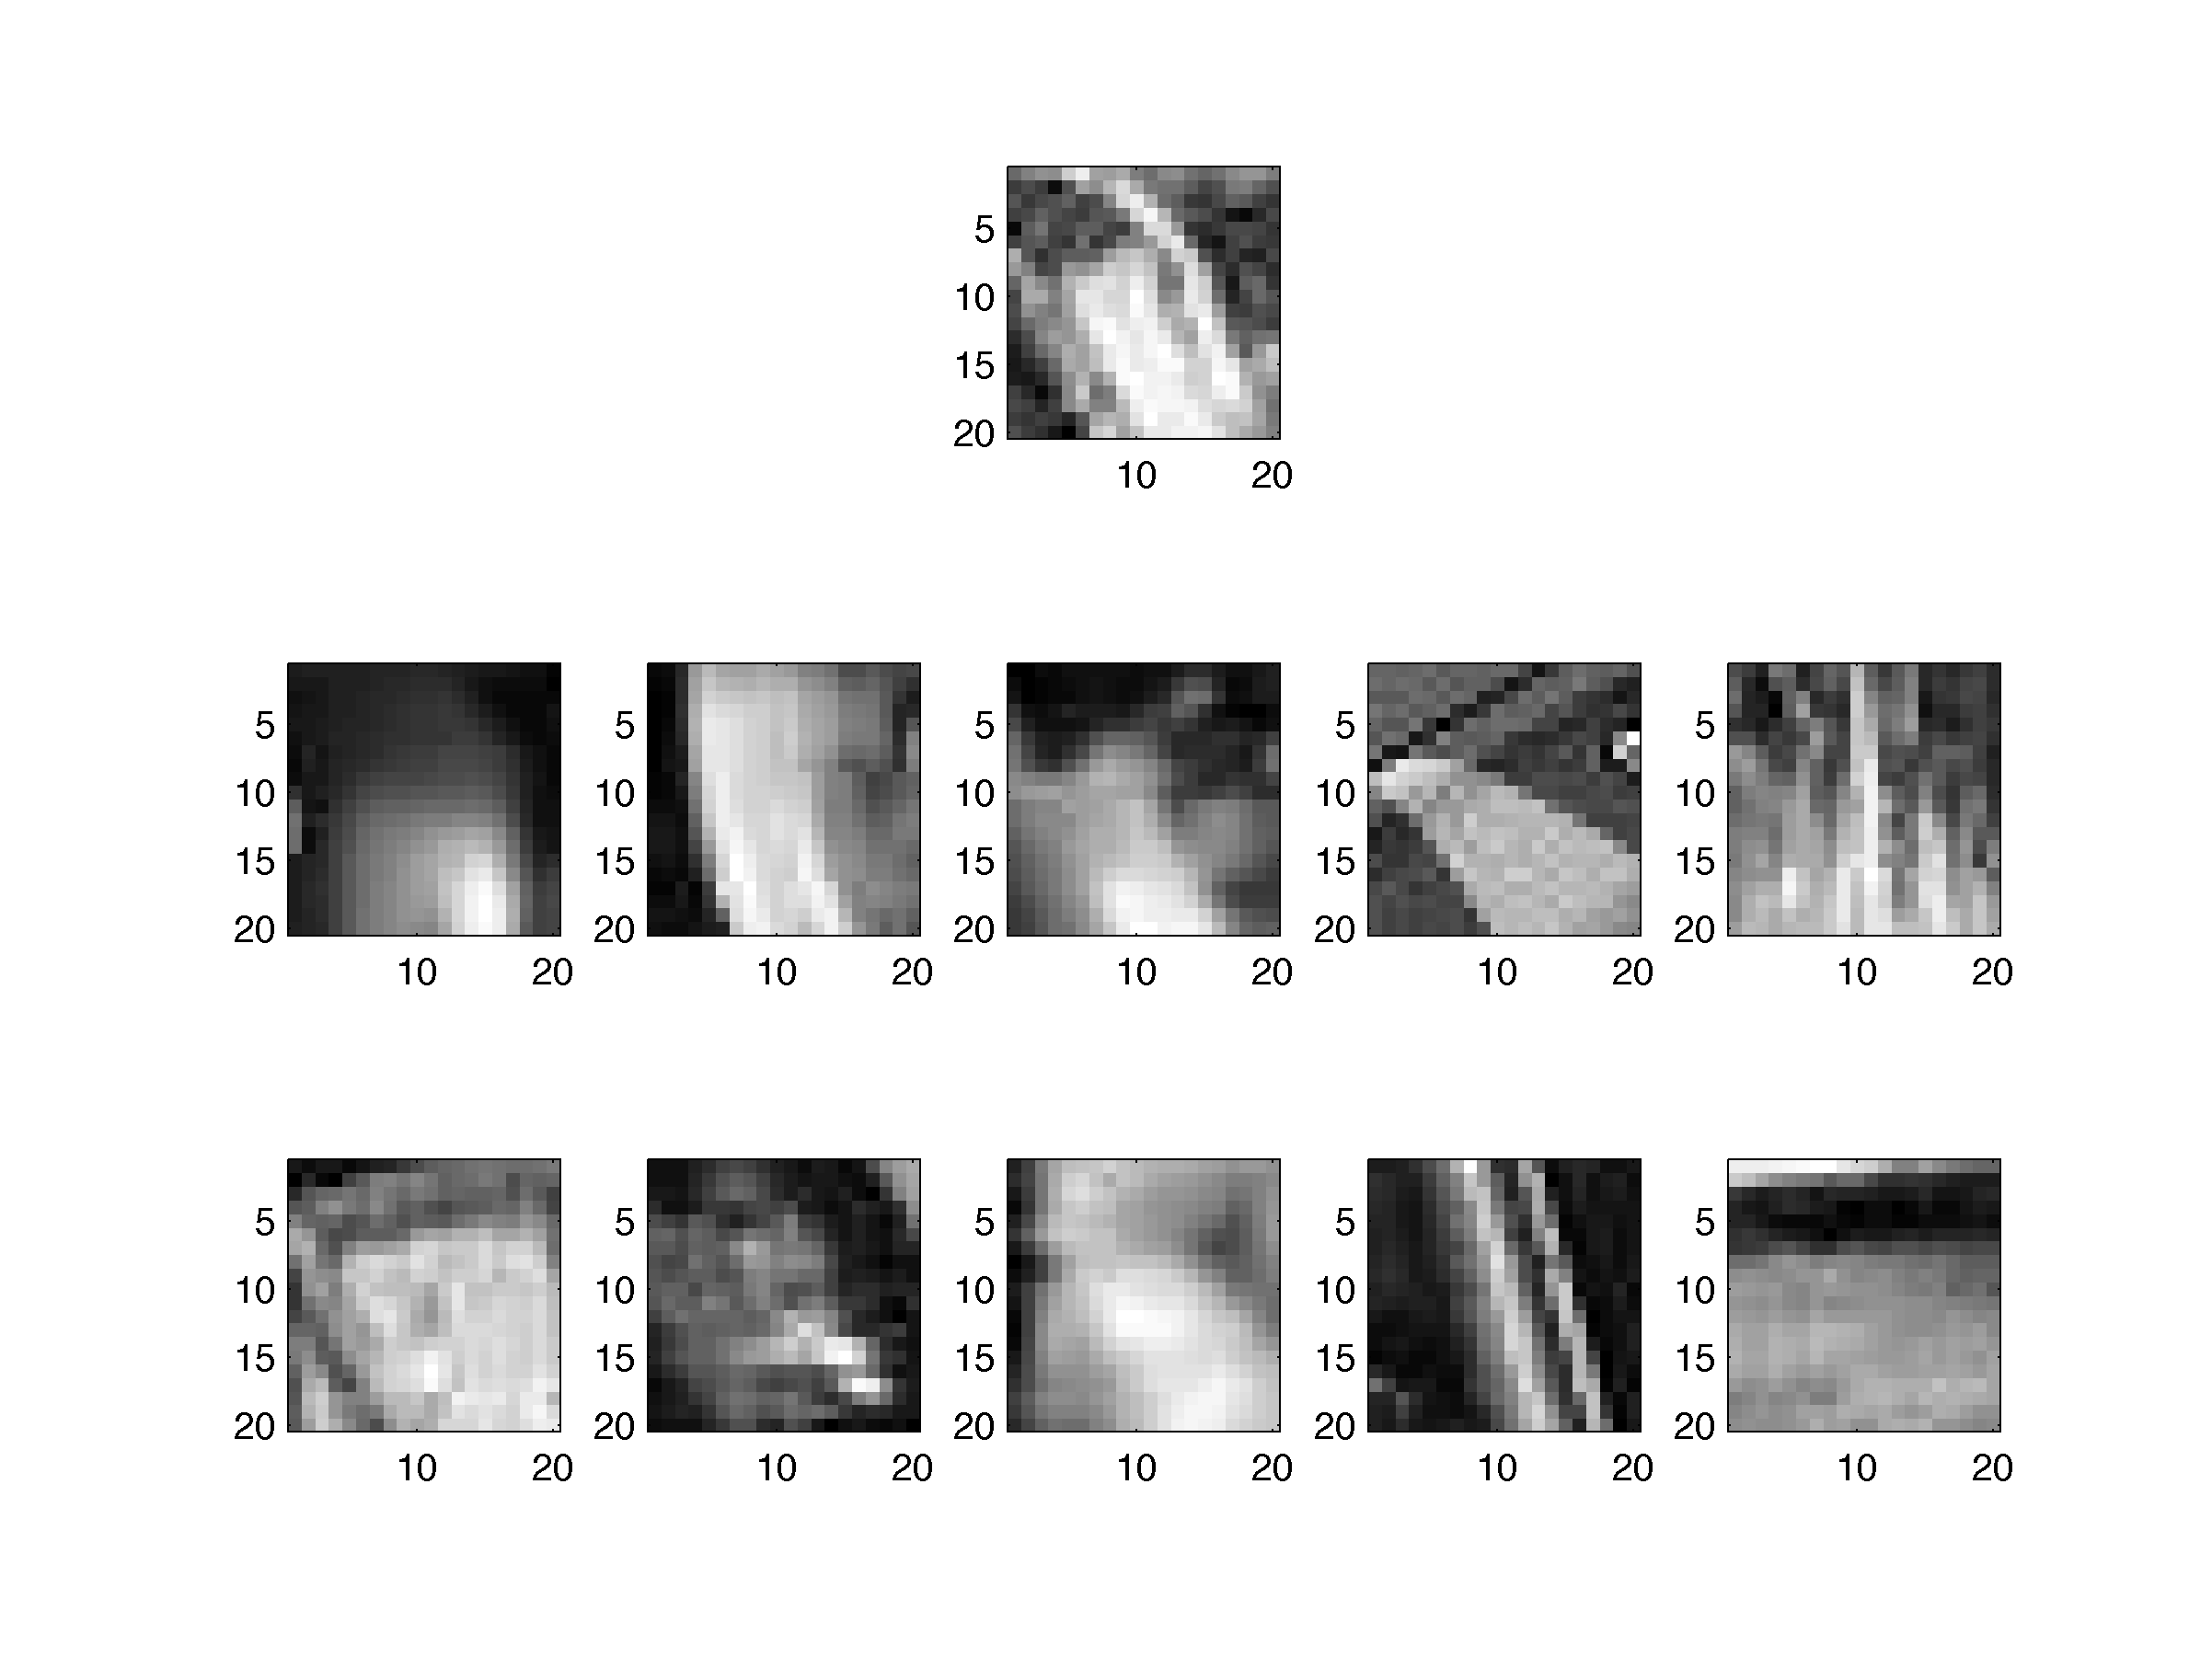
\includegraphics[scale=0.45]{linear_negihbor.png}
\caption{linear search}
\end{figure}


\end{document}

